% /solutions/conference-talks/conference-ornate-20min.fr.tex, 22/02/2006 De Sousa
\documentclass{beamer}
\usepackage{listings}
\usepackage{mdframed}
\usepackage{tikz}
% Ce fichier est un exemple d'expos\'e

% - pour des conf\'erences,
% - d'une dur\'ee approximative de 20 minutes,
% - avec un style ornemental.


% Copyright 2004 by Till Tantau <tantau@users.sourceforge.net>.
%
% Traduction de Philippe De Sousa <philippejjg@free.fr>
%
% En principe, ce fichier peut être redistribu\'e et/ou modifi\'e conform\'ement
% aux termes de la GNU Public License, version 2.
%
% Cependant, ce fichier est suppos\'e comme \'etant un "exemple-type" qui peut être modifi\'e
% selon vos propres besoins. Pour cette raison, si vous utilisez ce fichier en tant qu'
% "exemple-type" et non sp\'ecifiquement pour le distribuer en tant que partie d'un
% package ou programme, je vous donne la permission exceptionnelle de copier librement et
% de modifier ce fichier et même d'effacer ce message de copyright.
\usepackage{pdfpages}



\usepackage[francais]{babel}
% or autre comme par exemple \usepackage[english]{babel}

\usepackage[utf8]{inputenc}
% or autre

\usepackage{float}
\usepackage{graphicx}
\usepackage{wrapfig}
\usepackage{times}
\usepackage[T1]{fontenc}
% Or autre. Notez que le codage et la fonte doivent être assortis. Si T1
% ne paraît pas tr\`es esth\'etique, essayer d'effacer la ligne contenant fontenc.
\makeatletter
\hypersetup{pdfpagemode=FullScreen}

\mode<presentation> {
  \usetheme{UNLTheme}
  % ou autre ...
	
 	% \setbeamercovered{none}
  % ou autre chose (il est \'egalement possible de supprimer cette ligne)
}

\title[] % (facultatif, \`a utiliser uniquement si le titre de l'article est trop long)
{Logiciel de devis et Facturation}
\subtitle {FactDev}

\author[
\textbf{F}lorent\\
\textbf{A}ntoine\\
\textbf{C}édric\\
Manan\textbf{T}soa
] % (facultatif, \`a utiliser seulement avec plusieurs auteurs)
{Antoine de \bsc{Roquemaurel}\newline Florent \bsc{Berbie}\newline Cédric \bsc{Rohaut}\newline Manantsoa Andriamihary \bsc{Razanajatovo}}

% - Composez les noms dans l'ordre dans lequel ils apparaîtrons dans l'article
% - Utilisez la commande \inst{?} uniquement si les auteurs ont des affiliations
%   diff\'erentes.

\institute[] % (facultatif mais g\'en\'eralement n\'ecessaire)
{
  Universit\'e Toulouse III -- Paul Sabatier \\
  M1 Informatique -- Développement Logiciel 
  \vspace{-10px}
}
% - Utilisez la commande \inst uniquement s'il y a plusieurs affectations
% - Faîtes quelque chose de simple, personne ne s'int\'eresse \`a votre adresse

\date[ ~ ~ ~ JJ / MM / 2015] % (facultatif, peut être une abr\'eviation du nom de la conf\'erence)
{JJ / MM / 2015}
% - Utilisez \`a la fois le nom de la conf\'erence et son abr\'eviation.
% - N'a pas r\'eellement d'importance pour l'assistance qui sera pr\'esente lors de la conf\'erence,
%   mais en a surtout pour les personnes (y compris vous-même) qui liront les transparents en ligne.

\subject{Plateforme de tests automatis\'es}
% Ins\'er\'e uniquement dans la page d'information du fichier PDF. Peut être
% supprim\'e.


% Si vous avez un fichier nomm\'e "universit\'e-logo-nomfichier.xxx", où xxx
% est un format graphique accept\'e par latex ou pdflatex (comme par exemple .png),
% alors vous pouvez ins\'erer votre logo ainsi :

 \pgfdeclareimage[width=2.5cm]{le-logo}{../../images/FACT_official.png}
 \logo{\pgfuseimage{le-logo}}


% \`a supprimer si vous ne voulez pas que la table des mati\`eres apparaisse
% au d\'ebut de chaque sous-section : 
\AtBeginSection[] {
  \begin{frame}<beamer>{Plan}
    \tableofcontents[currentsection]
  \end{frame}
}
% Si vous souhaitez recouvrir vos transparents un \`a un,
% utilisez la commande suivante (pour plus d'info, voir la page 74 du manuel
% d'utilisation de Beamer (version 3.06) par Till Tantau) :

%\beamerdefaultoverlayspecification{<+->}


\setbeamertemplate{footline}{
	\leavevmode%
	\hbox{\hspace*{-0.6cm}
	\begin{beamercolorbox}[wd=.19\paperwidth,ht=2.25ex,dp=1ex,center]{section in head/foot}%
		\usebeamerfont{section in head/foot}\insertshortdate{}
	\end{beamercolorbox}%

	\begin{beamercolorbox}[wd=.76\paperwidth,ht=2.25ex,dp=1ex,center]{section in head/foot}%
		\insertprogressbar
		\usebeamerfont{section in head/foot} Développement d'un logiciel de facturation : FactDev 
		\end{beamercolorbox}%

		\begin{beamercolorbox}[wd=.10\paperwidth,ht=2.27ex,dp=1ex,right]{section in head/foot}%
			\usebeamerfont{section in head/foot}\hspace*{2em}
			\hspace{-10px}\textbf{\insertframenumber{}} / \inserttotalframenumber\hspace*{2ex}
		\end{beamercolorbox}}%
		\vskip0pt%
		}

		\setbeamertemplate{navigation symbols}{}
		\begin{document}
		\begin{frame}
			\titlepage
		\end{frame}
		\begin{frame}{Les parties prenantes}
			\begin{itemize}
				\item \'Equipe FACT
					\begin{itemize}
						\item {Antoine de \bsc{Roquemaurel}
						\item Florent \bsc{Berbie}
						\item Cédric \bsc{Rohaut}
						\item Manantsoa Andriamihary \bsc{Razanajatovo}}
					\end{itemize}
					\vfill
				\item Encadrant
					\begin{itemize}
						\item Frédéric \bsc{Migeon}
					\end{itemize}
					\vfill
				\item Client
					\begin{itemize}
						\item Antoine de \bsc{Roquemaurel}
					\end{itemize}
					\vfill
			\end{itemize}
		\end{frame}
		\begin{frame}
			\tableofcontents	
		\end{frame}
\section{Le projet} % Intro + Projet &=&  4'
\subsection{Le logiciel FactDev}
\begin{frame}{FactDev : Un logiciel de Devis et Facturation}
	\begin{block}{Un problème}
		\begin{itemize}
			\item Rédaction de factures et devis << à la main >> 
				\begin{itemize}
			\item Problème pour le calcul des montants
			\item Pour retrouver les factures dans les dossiers\\
				~$\Rightarrow$ Risque d'erreur humaine important
				\end{itemize}
		\end{itemize}
	\end{block}
	\vfill
	\begin{exampleblock}{Une solution}
		Un logiciel automatisant ce problème : 
	\begin{itemize}
		\item Gestion de clients, projets associés
		\item Calculs des Tarifs
		\item Génération de documents 
		\item Recherche
	\end{itemize}
	\end{exampleblock}
\end{frame}
\subsection{Les outils}
\begin{frame}{Les outils utilisés}
	\begin{figure}[H]
		\centering
		\uncover<1->{
			
\includegraphics[height=1.5cm]{logos/qt.png}~~
			\Huge \LaTeX
			
\includegraphics[height=0.8cm]{logos/sqlite.png}
		}

		\uncover<2->{
			
\includegraphics[height=1.0cm]{logos/git.png}~~
			
\includegraphics[height=0.8cm]{logos/github.png}
		}

		\uncover<3->{
			
\includegraphics[height=1.3cm]{logos/travis.png}~~
			
\includegraphics[height=1.3cm]{logos/coveralls.png}\\
			\vspace{-10px}
			
\includegraphics[height=0.5cm]{logos/doxygen.png}
		}

		\uncover<4->{
			
\includegraphics[height=0.8cm]{logos/irc.png}~~
			
\includegraphics[height=1.4cm]{logos/drive.png}~~
		}
		\vspace{-20px}
	\caption{Les différents outils}
\end{figure}
	%% Valgrind ? 
	
\end{frame}
\section{La méthodologie} %  Méthodo = 8'
\subsection{La méthode Scrum}
\begin{frame}{\large Scrum, une méthodologie de développement}
			\only<2>{
			\vspace{15px}
			}
	\begin{block}{Scrum : méthode agile}
		\begin{itemize}
			\item Incrémental
			\item Absence d'effet tunnel
		\end{itemize}
		\begin{figure}[H]
			\centering
			\vspace{-15px}
			\only<2>{
			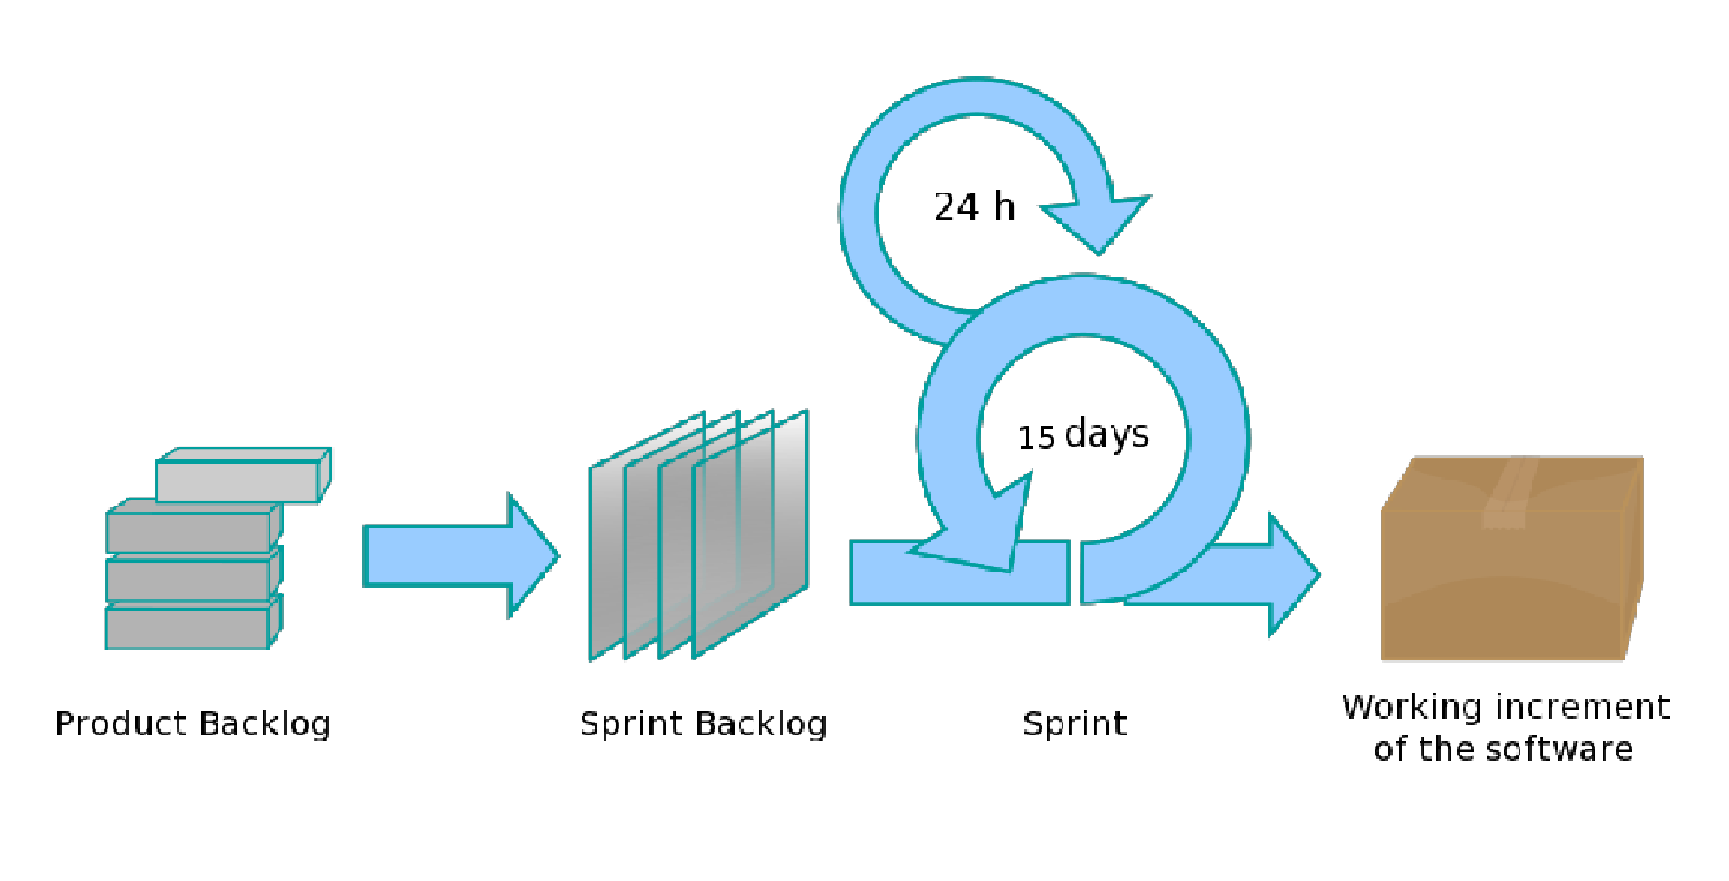
\includegraphics[width=5.8cm]{images/Scrum_process.eps}
			}
			\only<3->{
			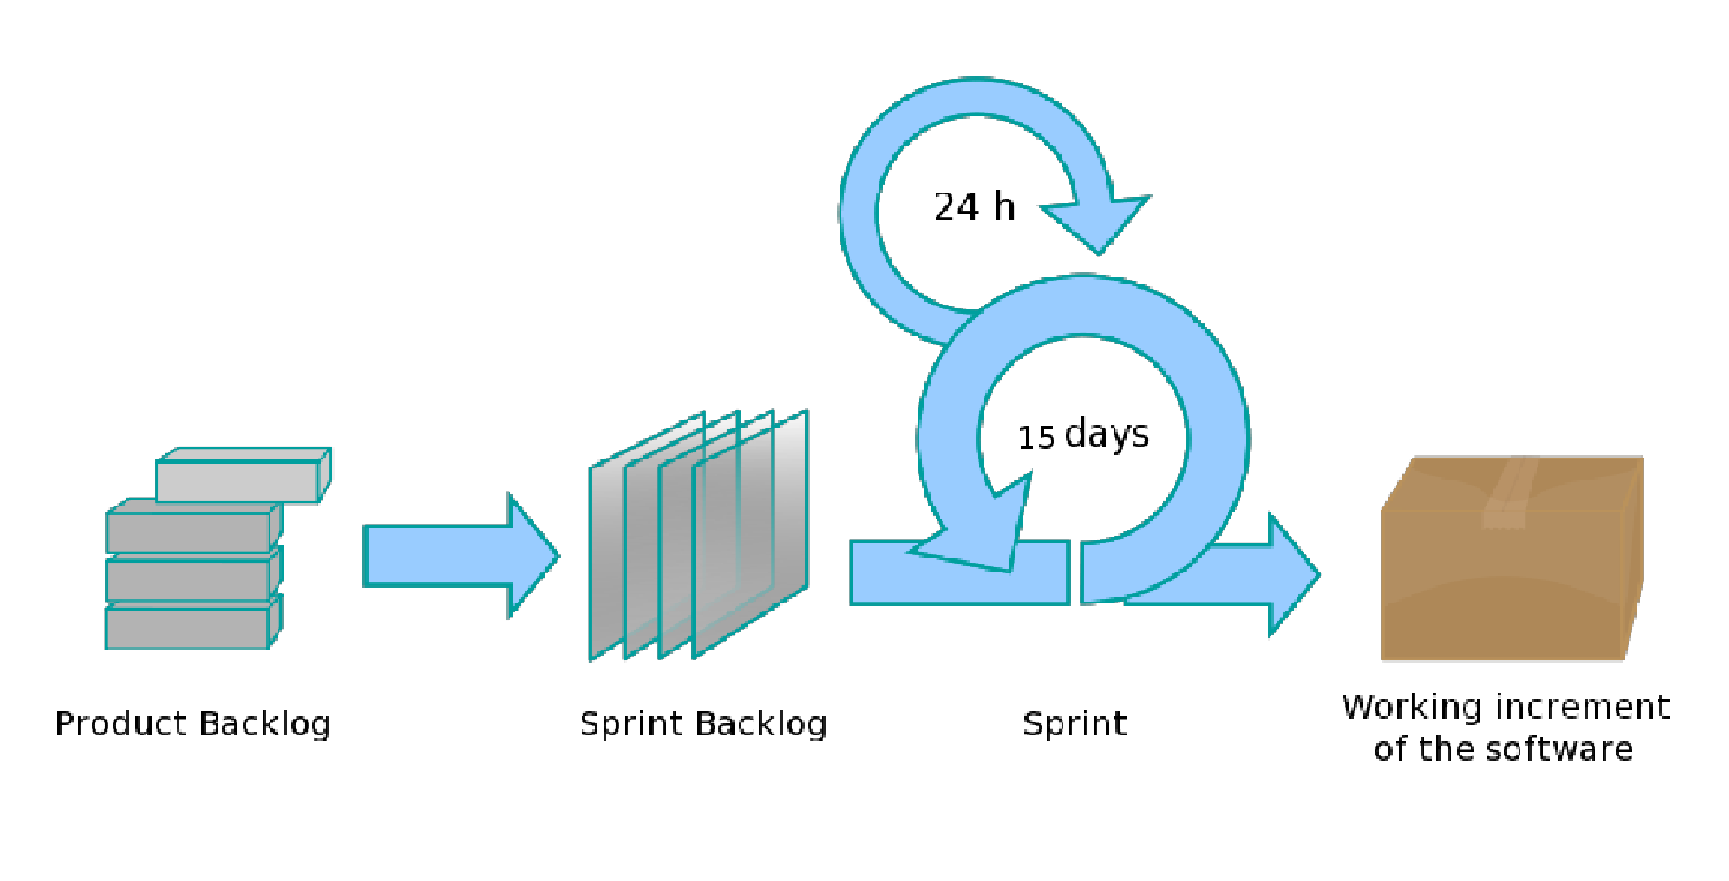
\includegraphics[width=2.8cm]{images/Scrum_process.eps}
			}
			\only<2->{
			\vspace{-10px}
			\caption{Processus de développement Scrum}
			}
		\end{figure}
	\end{block}
	\uncover<3->{
	\begin{block}{User Stories}
		\begin{itemize}
			\item Fonctionnalités
			\item Finie
				\begin{itemize}
					\item 
\includegraphics[height=7px]{images/coverage.png}~~Couverture de code > 80\% % TODO image
					\item 
\includegraphics[height=7px]{images/build.png}~~Build passing % TODO image 
					\item \texttt{// Code documenté}
					\item 
\includegraphics[height=9px]{images/pullrequest.png}~~Code relu et validé par une tierce personne
				\end{itemize}
		\end{itemize}
	\end{block}
	}
\end{frame}
\begin{frame}{\large Scrum, une méthodologie de développement}
	\begin{block}{Organisation}
		\begin{tabular}{cc}
		\begin{minipage}{0.36\textwidth}
	\setbeamercovered{transparent}{
		\begin{itemize}
			\item<1,4-> Backlog
			\item<2,4-> Planning Poker
			\item<3,4-> Mêlées
		\end{itemize}
}
	\end{minipage}&
	\begin{minipage}{0.6\textwidth}
		\begin{figure}[H]
			\only<1>{
			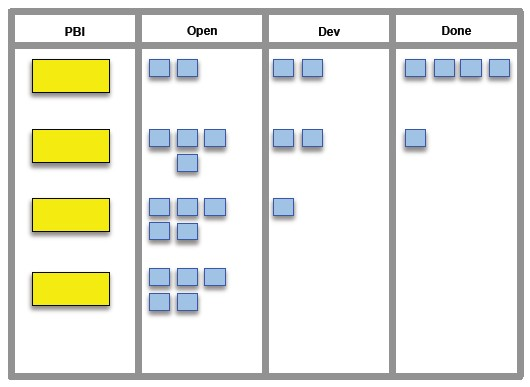
\includegraphics[height=2.5cm]{images/backlog.jpg}
			}
			\only<2>{
			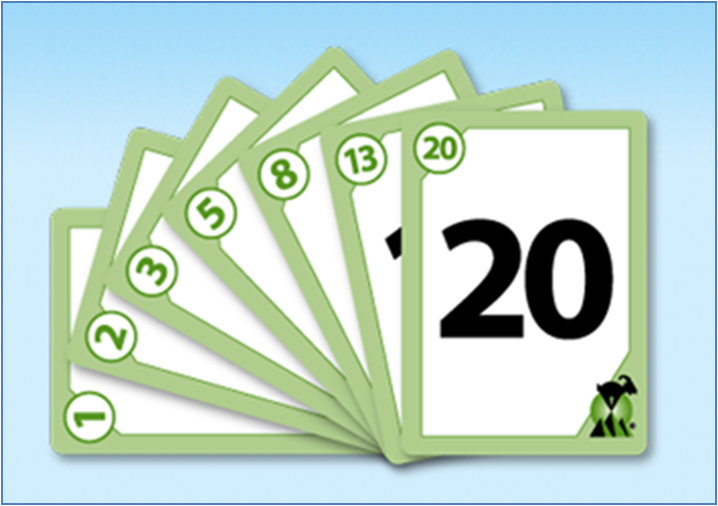
\includegraphics[height=2.5cm]{images/cards-planning-poker.png}
			}
			\only<3>{
			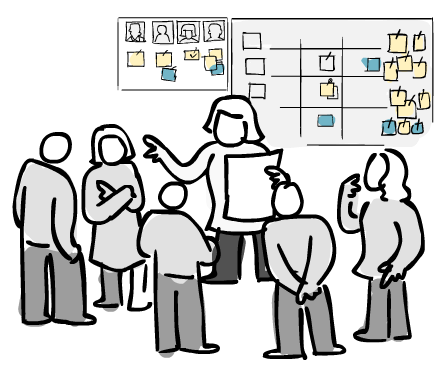
\includegraphics[height=2.5cm]{images/melees.png}
			}
			\only<4->{
			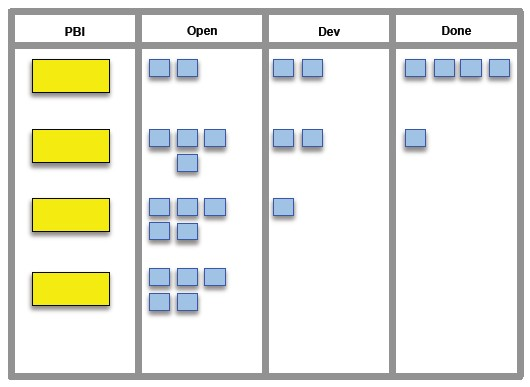
\includegraphics[height=1.2cm]{images/backlog.jpg}~
			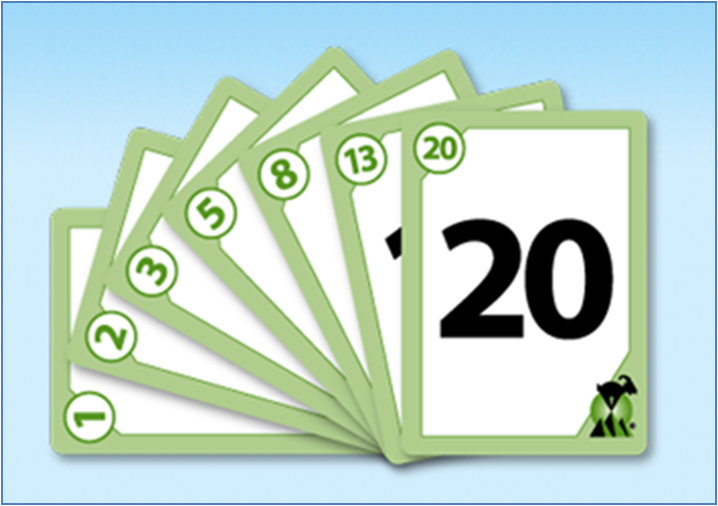
\includegraphics[height=1.2cm]{images/cards-planning-poker.png}~
			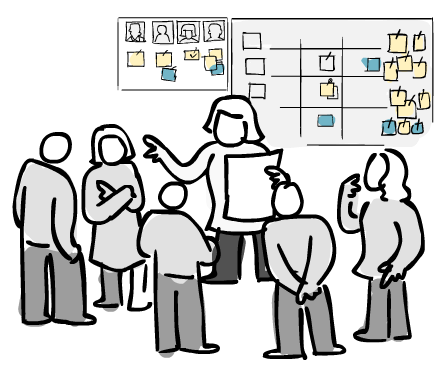
\includegraphics[height=1.2cm]{images/melees.png}
			}
		\end{figure}
	\end{minipage}
\end{tabular}
	\end{block}
	\uncover<4->{
	\begin{block}{Les différents rôles}
		\begin{tabular}{cc}
		\begin{minipage}{0.36\textwidth}
	\setbeamercovered{transparent}{
		\begin{itemize}
			\item<5> Scrum Master
			\item<6> Product Owner
			\item<7> Responsable technique
			\item<8> Équipe de développement
		\end{itemize}
		}
	\end{minipage}&
	\begin{minipage}{0.6\textwidth}
		\begin{figure}[H]
			\centering
			\only<5>{
			
\includegraphics[height=2.5cm]{images/photos/kratux.png}
			}
			\only<6-7>{
			
\includegraphics[height=2.5cm]{images/photos/satenske.png}
			}
			\only<8>{
			
\includegraphics[height=1.5cm]{images/photos/kratux.png}~
			
\includegraphics[height=1.5cm]{images/photos/satenske.png}\newline
			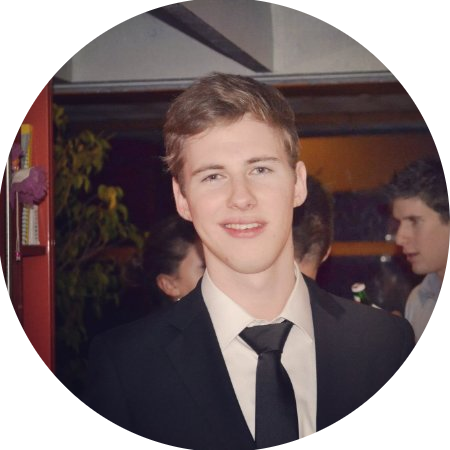
\includegraphics[height=1.5cm]{images/photos/oxynos.png}~
			
\includegraphics[height=1.5cm]{images/photos/tsoo.png}
			}
		\end{figure}
	\end{minipage}
\end{tabular}
	\end{block}
	}
\end{frame}
% Pull Requests	
% Branching flow
\subsection{L'intégration continue}
\begin{frame}{Intégration\ldots}
	\begin{block}{Git et Github}
		\begin{tabular}{cc}
			\begin{minipage}{0.5\textwidth}
				\begin{itemize}
						\uncover<1->{
					\item Contrôle de version 
					\item Fusion automatique
						}
						\uncover<2->{
					\item Communication
					\item Issues
						}
				\end{itemize}
			\end{minipage} & 
			\begin{minipage}{0.48\textwidth}
				\begin{figure}[H]
					\hspace{-49px}
					\uncover<1->{
					\vspace{25px}
						
\includegraphics[height=1.6cm]{logos/gitvertical.png}~
					}
					\uncover<2->{
						
\includegraphics[height=1.6cm]{logos/githubvertical.png}
					}
				\end{figure}
			\end{minipage}
		\end{tabular}
	\end{block}
\end{frame}
\begin{frame}{Intégration\ldots}
	\begin{figure}[H]
		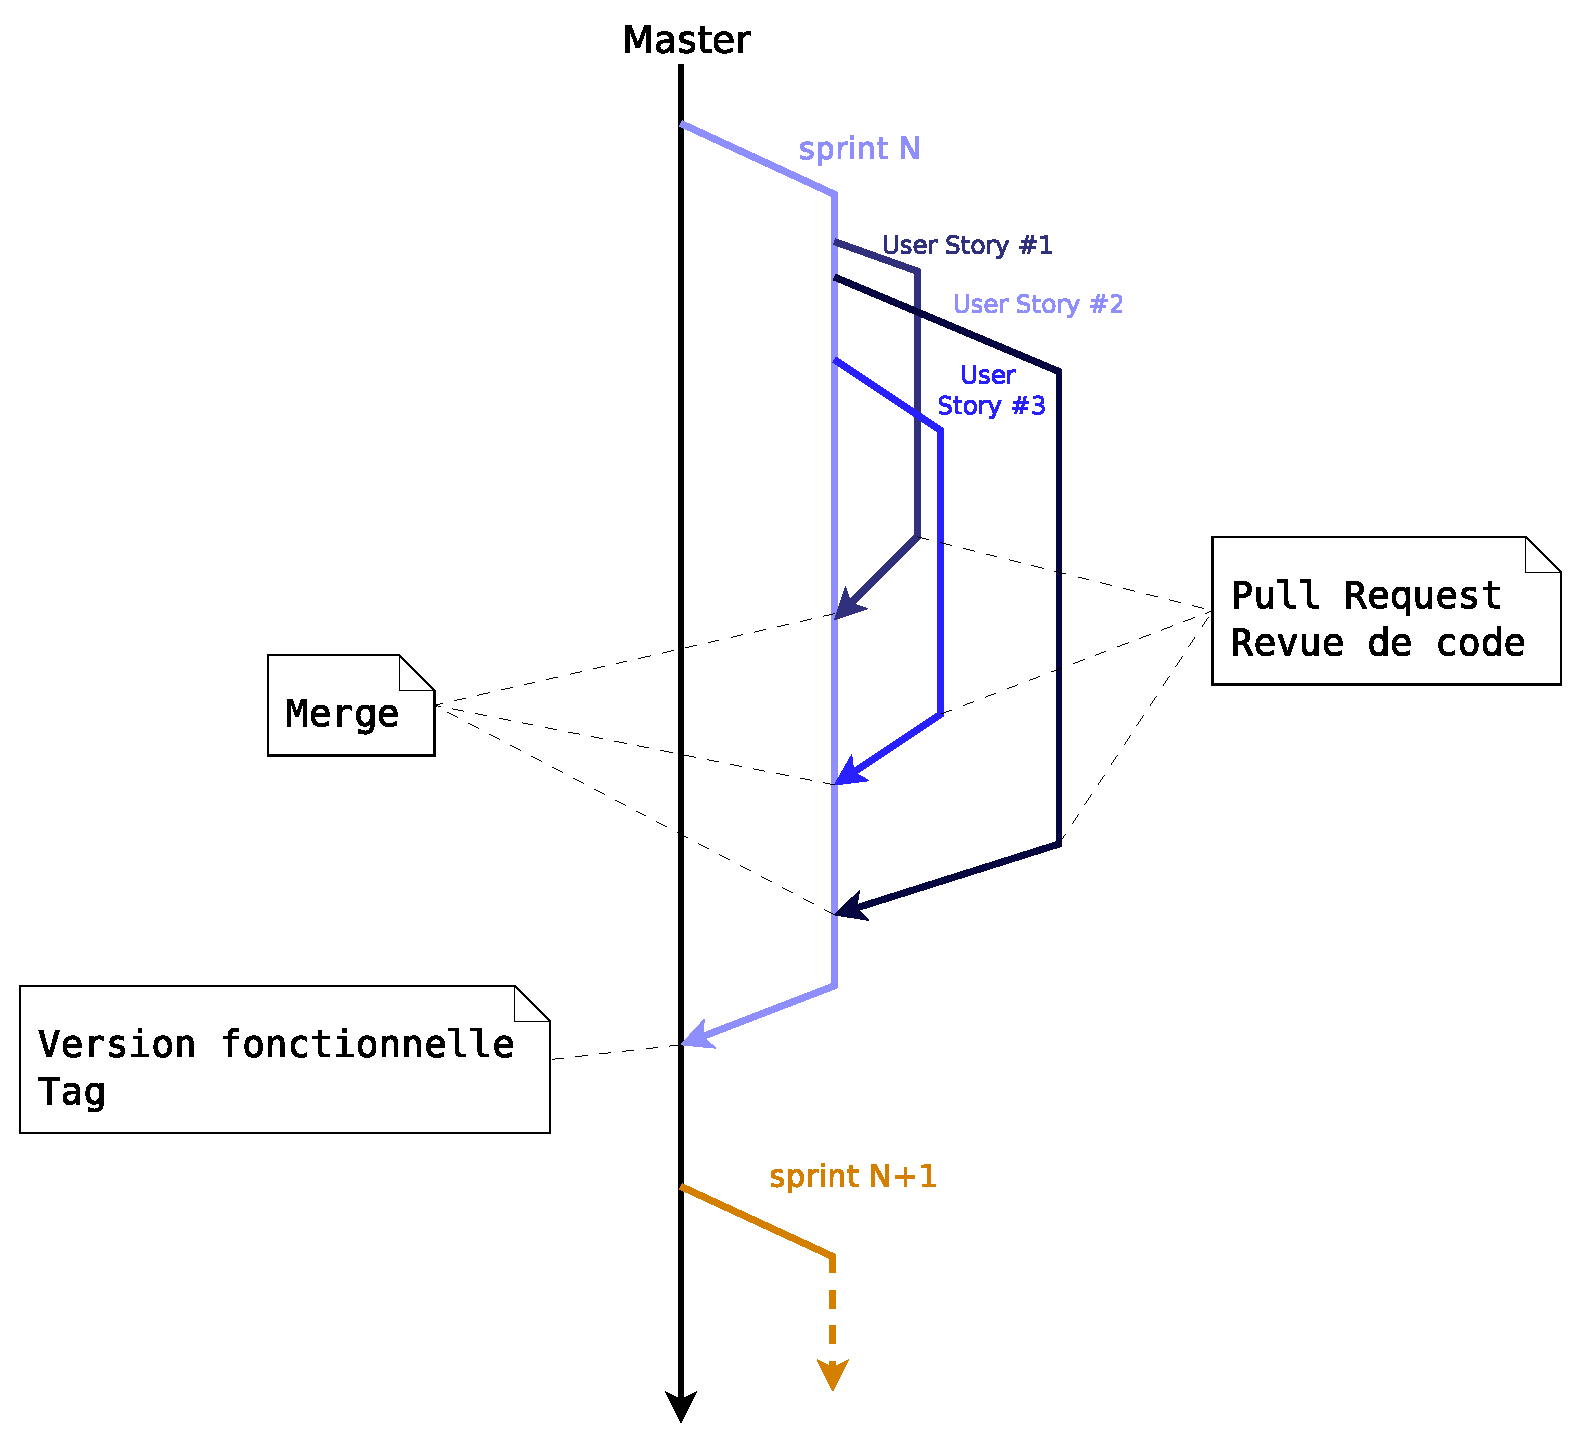
\includegraphics[height=7.5cm]{images/BranchingWorkflow.eps}
		\vspace{-10px}
		\caption{Git Branching}
	\end{figure}
\end{frame}

\begin{frame}{\ldots Continue}
	\begin{figure}[H]
		\centering
		\only<1>{
			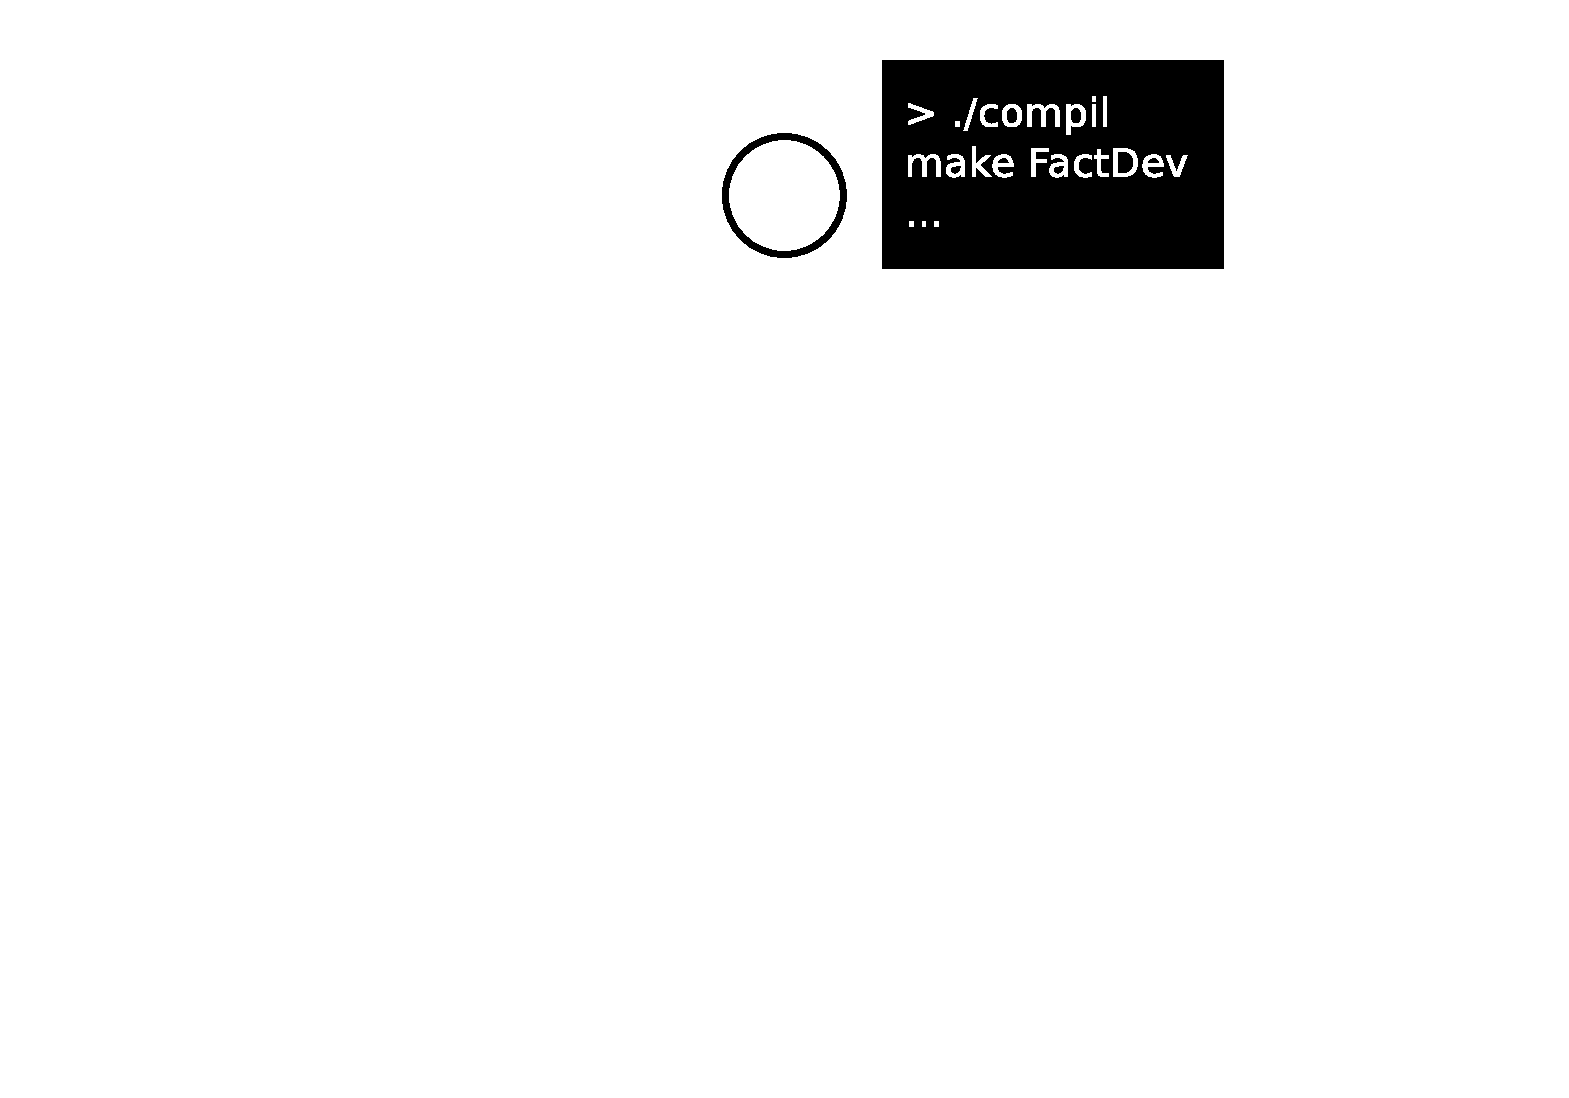
\includegraphics[width=9cm]{images/Travis/travis1_compil.eps}
		}
		\only<2>{
			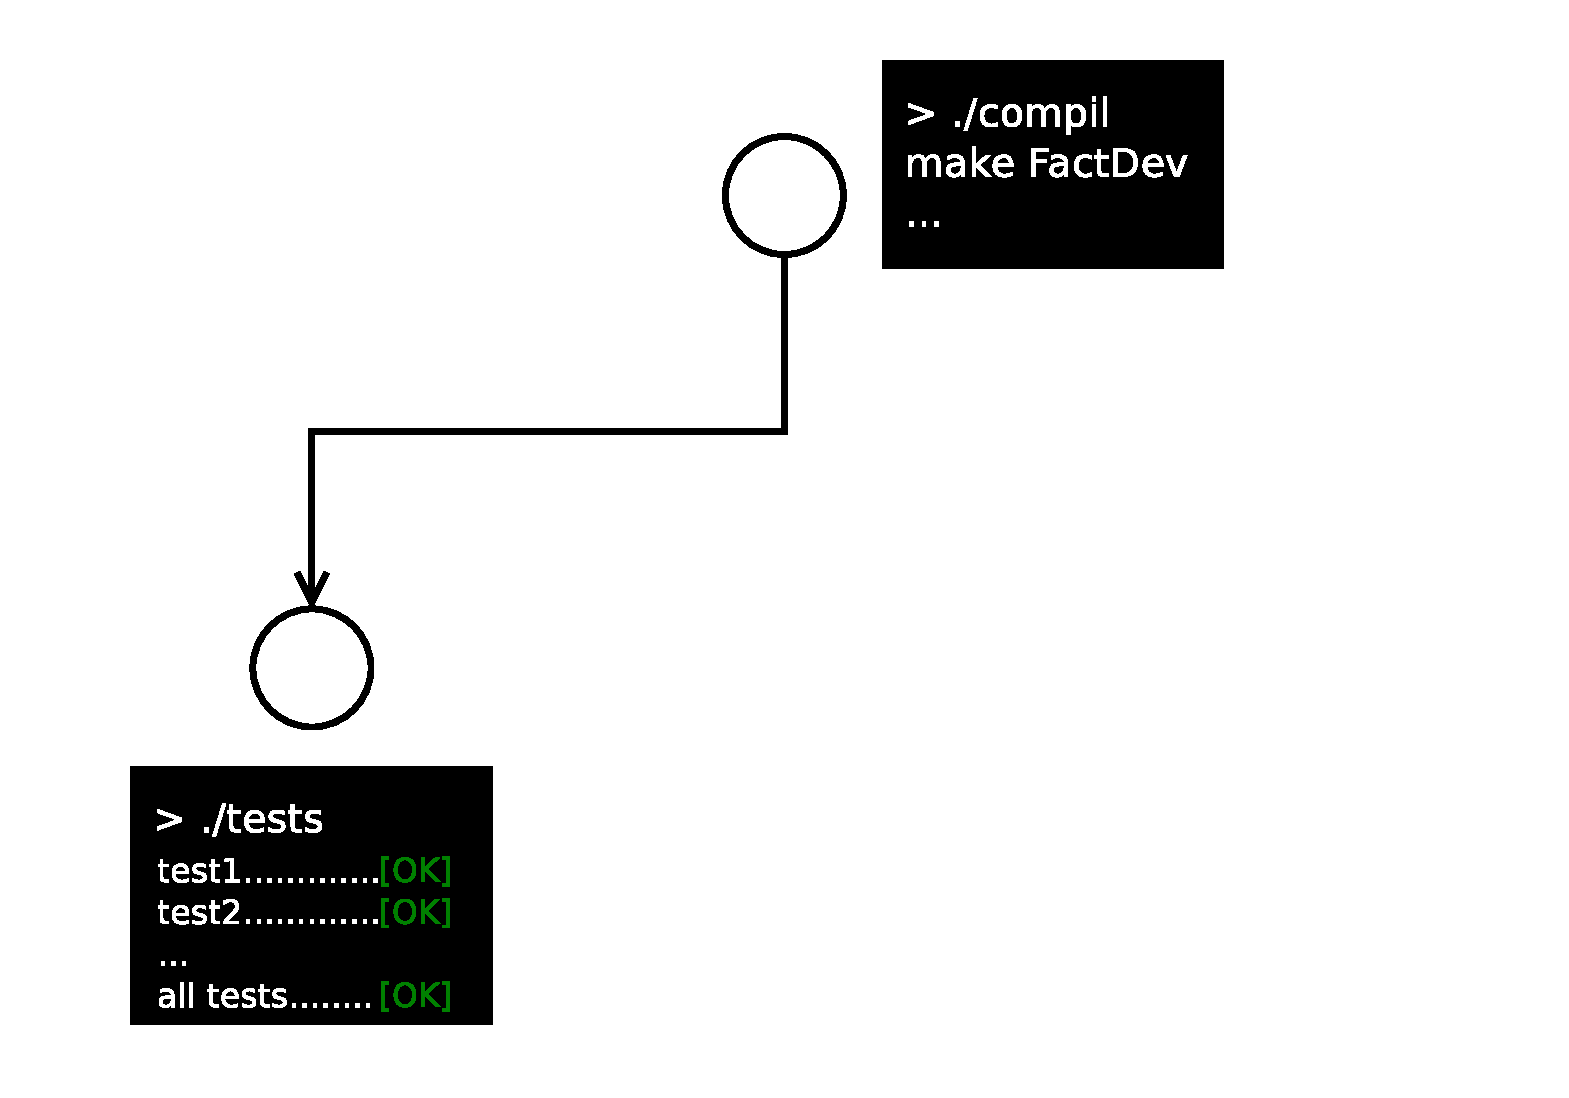
\includegraphics[width=9cm]{images/Travis/travis2_tests.eps}
		}		
		\only<3>{
			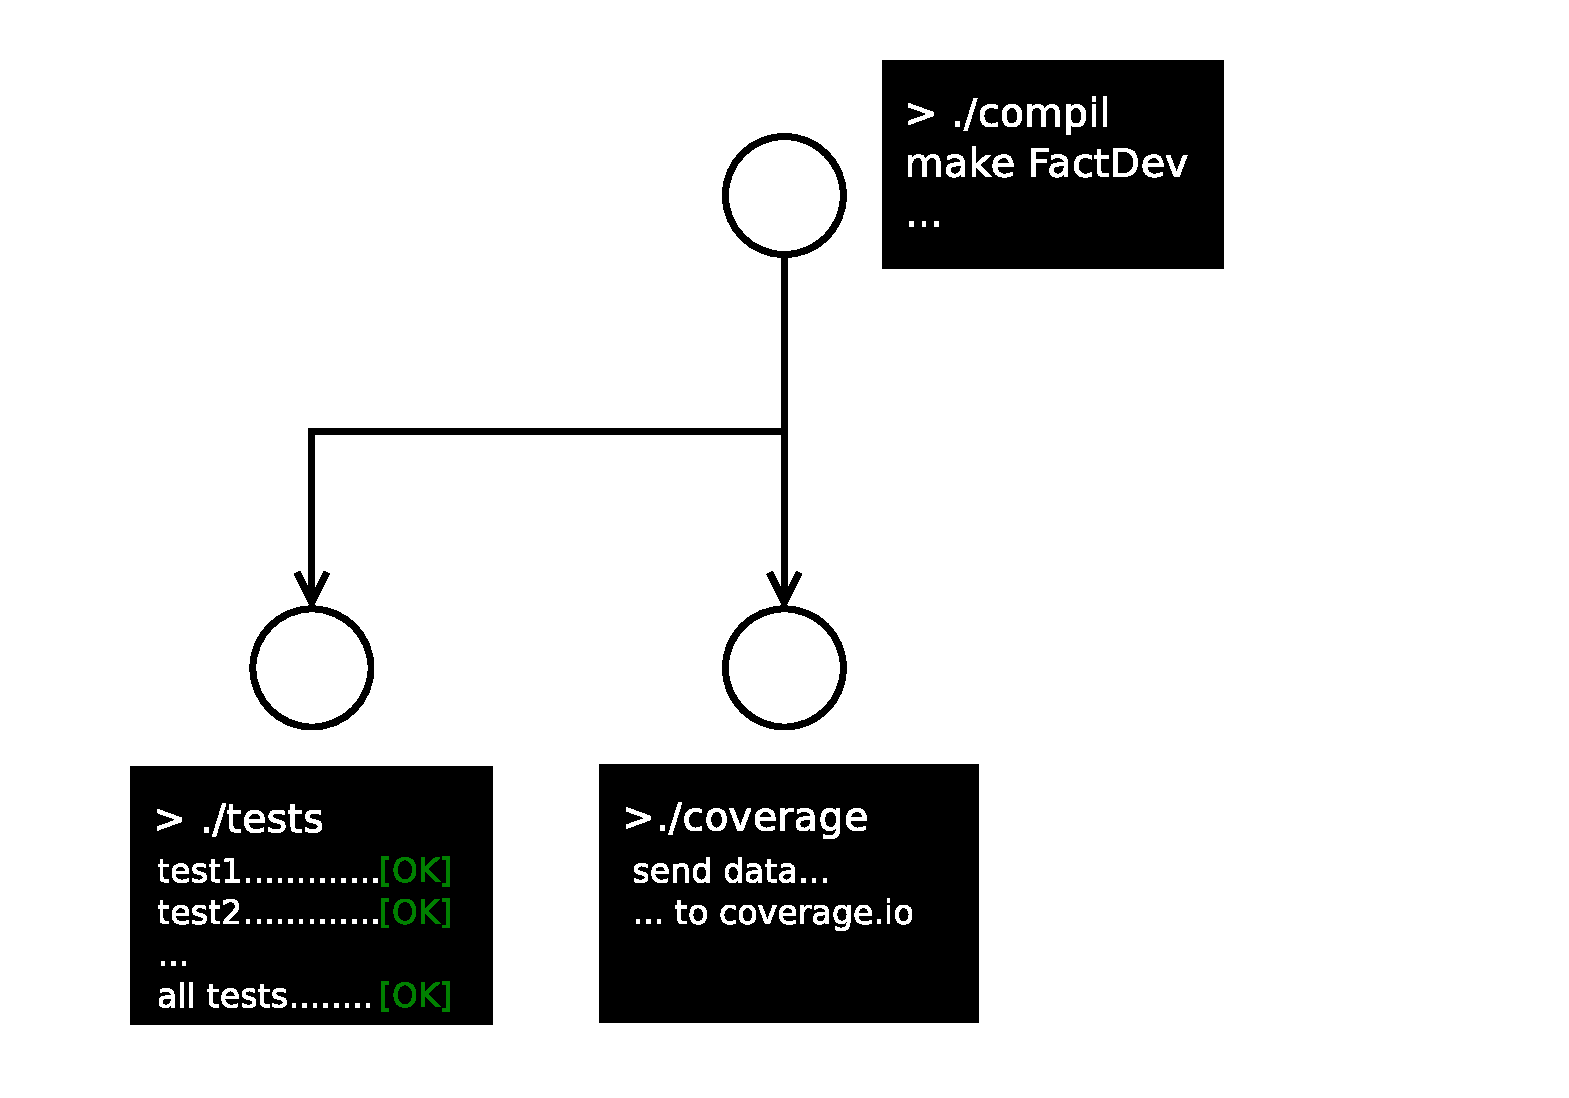
\includegraphics[width=9cm]{images/Travis/travis3_coverage.eps}
		}	
		\only<4>{
			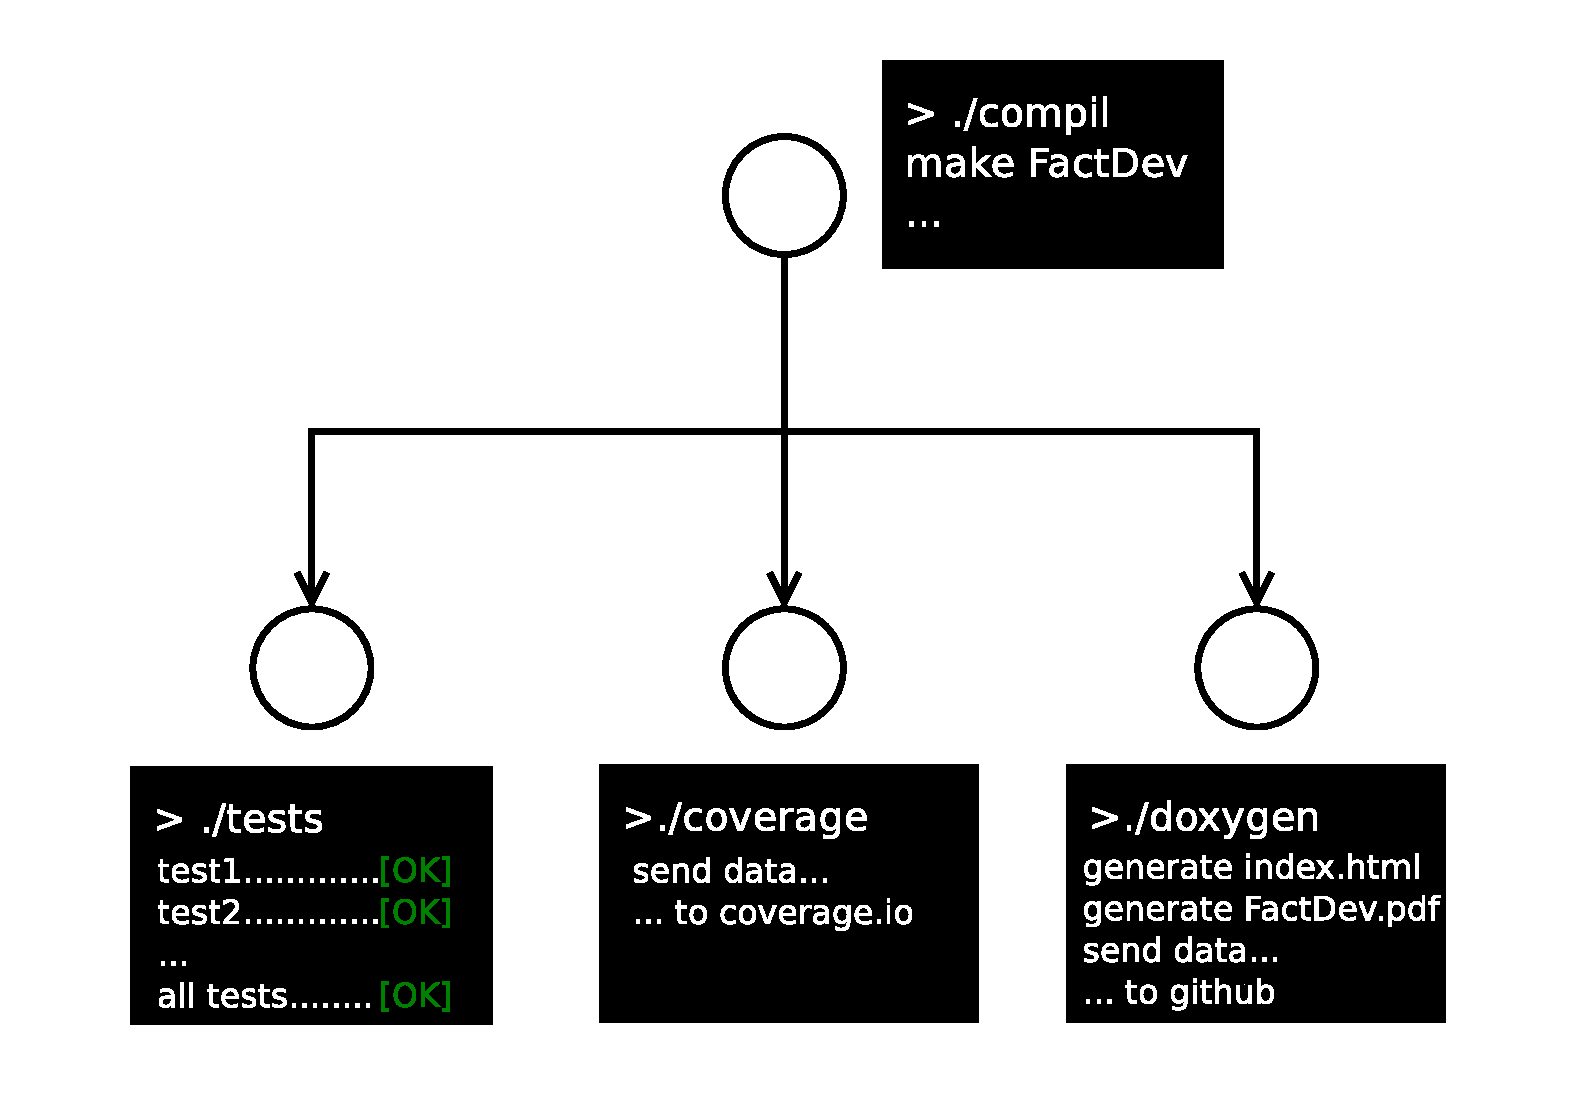
\includegraphics[width=9cm]{images/Travis/travis4_doxygen.eps}
			\newline 
			
\includegraphics[height=8px]{images/build.png} 
		}	
		\only<5>{
			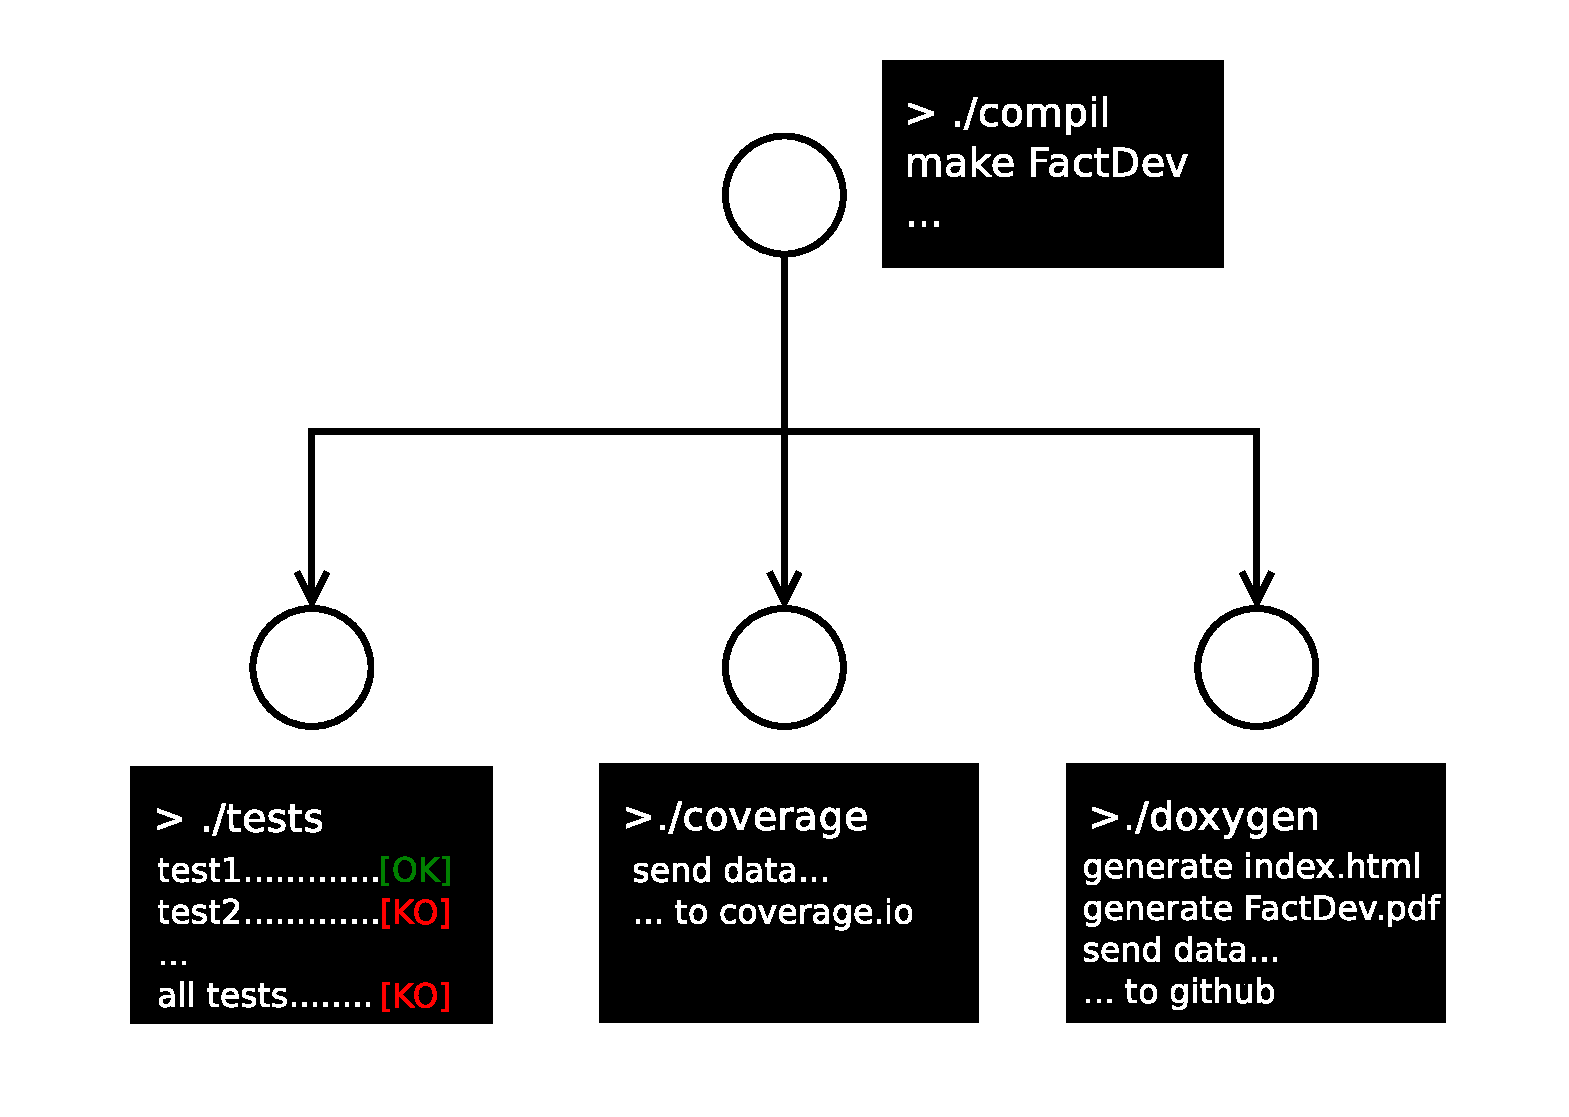
\includegraphics[width=9cm]{images/Travis/travis5_fail.eps}
			\newline 
			
\includegraphics[height=8px]{images/build_failing.png} 
		}
		
		\caption{Intégration continue avec Travis CI}
	\end{figure}

% Couverture de code
% Build, 
% Tests
% Transition vers la revue de code :)

\end{frame}
\subsection{La revue de code}
\begin{frame}{Vers 100\% de revue de code}
\begin{itemize}
\item Toutes intégrations nécessitent une \textbf{Pull Request}
\end{itemize}
\vfill
\pause
\begin{block}{\normalsize Validation d'une Pull Request par une tierce personne}
	\begin{itemize}
		\item Le code
			\begin{itemize}
				\item Est lisible
				\item Est compréhensible
				\item Respecte les conventions d'écriture
			\end{itemize}
		\item Les tests fonctionnels sont validés
		\item Le code est documenté
		\item 
\includegraphics[height=7px]{images/all_is_well.png}
		\begin{itemize}
		\item Le build passe
		\item Pas de régression de la couverture de code
	\end{itemize}
	\end{itemize}
\end{block}	
\end{frame}
\section{Les résultats} % Résultats = 5'
\subsection{La méthodologie}
\begin{frame}{Quelques chiffres\ldots}
	\begin{block}{Github}
		\begin{tabular}{cc}
			\hspace{-20px}
			\begin{minipage}{0.56\textwidth}
				\begin{itemize}
					\item 
\includegraphics[height=10px]{images/labels/pullRequestGreen.JPG}~Pull Requests~
\includegraphics[height=10px]{images/stats/pullrequest.png}
					\item 
\includegraphics[height=10px]{images/labels/issues.JPG}~Issues~
\includegraphics[height=10px]{images/stats/issues.png}
				\end{itemize}
			\end{minipage}
			\hspace{-15px}
			\begin{minipage}{0.5\textwidth}
				\begin{itemize}
					\item 
\includegraphics[height=10px]{images/labels/branches.JPG}~Branches~
\includegraphics[height=10px]{images/stats/branches.png}
					\item 
\includegraphics[height=10px]{images/labels/commits.JPG}~Commits~
\includegraphics[height=10px]{images/stats/commits.png}
				\end{itemize}
			\end{minipage}
		\end{tabular}
	\end{block}
\pause
	\begin{block}{Scrum}
		\begin{itemize}
			\item 54 User stories
			\item 6 sprints
			\item 2 releases
		\end{itemize}
	\end{block}
\pause
	\begin{block}{Code}
		\begin{itemize}
			\item Nombre de lignes 
\includegraphics[height=9px]{images/stats/nblines.jpg}
			\item 
\includegraphics[height=7px]{images/coverage.png}~~
\includegraphics[height=7px]{images/build.png}
			\item Pourcentage documentation
		\end{itemize}
	\end{block}

\end{frame}

\begin{frame}{BurnUp Chart}
	\begin{figure}[H]
		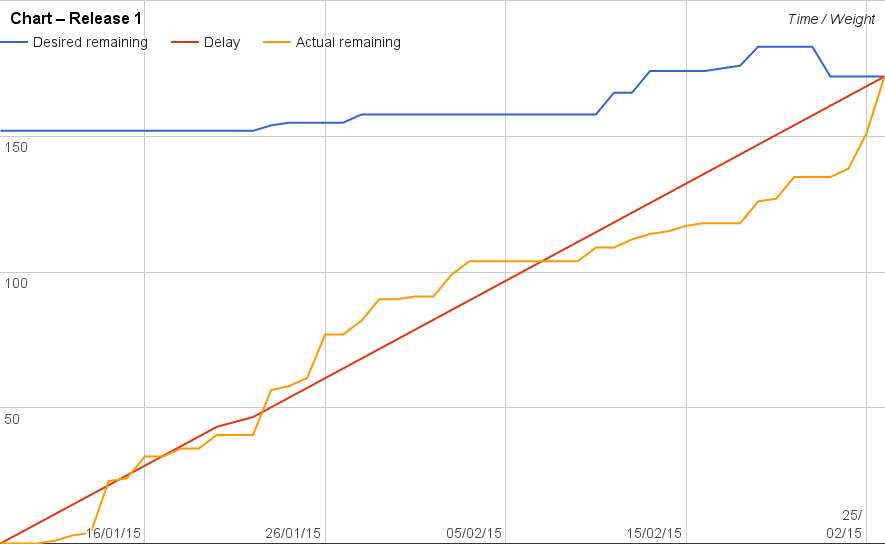
\includegraphics[width=9.5cm]{images/release1Chart.png}
		\caption{Première release}
	\end{figure}
\end{frame}

\subsection{Le logiciel}
\begin{frame}
% Screens 
\end{frame}

\section*{Conclusion} % 3'
\begin{frame}
% It was cool. But difficult. But we learn. And it was cool. And ? 
	
\end{frame}

% Slide for questions
\begin{frame}{Avez-vous des questions ?}
	\begin{figure}[H]
		\centering
		
\includegraphics[width=5cm]{interrogation.png}
	\end{figure}
\end{frame}
\end{document}
